\subsection{Ετερογενής Αρχιτεκτονική}
\subparagraph{}
Η ετερογενής αρχιτεκτονική είναι ένα σύνολο προδιαγραφών που επιτρέπουν την ενσωμάτωση κεντρικών μονάδων επεξεργασίας και επεξεργαστών γραφικών στον ίδιο δίαυλο, με κοινόχρηστη μνήμη και διεργασίες\cite{toms_hardware}.

Εξειδικευμένη επεξεργαστές επιταχυντών που βελτιώνουν δραματικά την απόδοση υπολογισμών, πολλαπλασιάζονται και οι επεξεργαστές γενικής χρήσης συνδέονται σε κάποιον επιταχυντή. Η αύξηση της δημοτικότητας αυτών των ετερογενών αρχιτεκτονικών σε όλους τους τύπους υπολογιστών είχε αξιοσημείωτο αντίκτυπο στην ανάπτυξη λογισμικού.

Για την εκμετάλλευση αυτών των συστημάτων, οι χρήστες πρέπει να κατασκευάζουν λογισμικό που εκτελεί διάφορες περιοχές κώδικα σε διαφορετικούς τύπους συσκευών. Το μεγαλύτερο κίνητρο αποτελεί η επιτάχυνση των υπολογισμών στους βρόγχους επανάληψης.

Ωστόσο, τα μοντέλα προγραμματισμού για αυτά τα συστήματα είναι δύσκολο να χρησιμοποιηθούν. Συχνά, οι ενότητες κώδικα γράφονται δύο φορές, μία φορά για τον επεξεργαστή γενικού σκοπού και μια για τον επιταχυντή. Η έκδοση του επιταχυντή γράφεται γλώσσα χαμηλότερου επιπέδου.
Τα παραπάνω προβλήματα οδηγούν σε δυσκολία συντήρησης λογισμικού και ανάγκη διατήρησης δύο εκδόσεων ίδιου κώδικα.

Για τις ανάγκες διευκόλυνσης, το \emph{\en{OpenMP}} επέκτεινε τις λειτουργίες του με σκοπό να υποστηρίξει αυτούς τους τύπους συστημάτων\cite{barbara}. Τα αποτελέσματα της εργασίας αρχικά δημοσιεύτηκαν στην έκδοση 4.0 και στη ανανεώθηκαν στην έκδοση 4.5.

Ο χρήστης μπορεί να χρησιμοποιήσει την διεπαφή \emph{\en{OpenMP}}, για να προγραμματίσει επιταχυντές σε υψηλότερο επίπεδο γλώσσας και για τη διατήρηση μίας μόνο έκδοσης του κώδικα, η οποία μπορεί να τρέξει είτε σε επιταχυντή είτε σε επεξεργαστή γενικής χρήσης.

Κίνητρο για την εκτέλεση κώδικα σε μια ετερογενή αρχιτεκτονική είναι να εκτελεστεί ένα κομμάτι κώδικα σε έναν επιταχυντή. Ο ρόλος των επιταχυντών είναι η δραματική βελτίωση της απόδοσης ενός προγράμματος αξιοποιώντας τις δυνατότητες υλικού των συσκευών αυτών. Το \emph{\en{OpenMP}} παρέχει τα μέσα για τη διανομή εκτέλεσης ενός προγράμματος σε διαφορετικές συσκευές με ετερογενή αρχιτεκτονική. Συσκευή είναι ένας υπολογιστικός πόρος όπου μια περιοχή κώδικα μπορεί να εκτελεστεί. Παραδείγματα τέτοιων συσκευών είναι GPU, CPU, DSP, FPGA κ.α.

Οι συσκευές έχουν τα δικά τους νήματα, των οποίων η μετεγκατάσταση σε άλλες συσκευές δεν είναι δυνατή. Η εκτέλεση του προγράμματος ξεκινάει από την κεντρική συσκευή (\emph{\en{host device}}. Η κεντρική συσκευή είναι υπέυθυνη για την μεταφορά του κώδικα και των δεδομένων στον επιταχυντή.

\selectlanguage{english}
\begin{lstlisting}[language=C++, caption={\el{Παράδειγμα} taskwait} , frame=tlrb]{Name}
 void add_arrays(double *A, double *B, double *C, size_t size) {
     size_t i = 0;
 #pragma omp target map(A, B, C)
     for (i = 0; i < size; ++i) {
             C[i] = A[i] + B[i];
     }
 }
\end{lstlisting}
\selectlanguage{greek}

Οταν ένα νήμα του εξυπηρετητή συναντάει την οδηγία \emph{\en{target}}, η περιοχή που ακολουθεί εκτελείται σε έναν επιταχυντή. Απο προεπιλογή, το νήμα που συναντά την οδηγία περιμένει την ολοκλήρωση της εκτέλεσης της παράλληλης περιοχής, προτού συνεχίσει.

Πριν το νέο νήμα αρχίσει να εκτελεί την παράλληλη περιοχή, οι μεταβλητές  \emph{\en{A, B, C}} αντιστοιχίζονται στον επιταχυντή. Η φράση \emph{\en{mapped}} είναι η έννοια που χρησιμοποιεί το \emph{\en{OpenMP}} για να περιγράψει τον τρόπο κοινής χρήσης των μεταβλητών σε όλες τις συσκευές.



\subsubsection{Το αρχικό νήμα της συσκευής προορισμού}
\subparagraph{}
Το νήμα που ξεκινάει την εκτέλεση ενός προγράμματος και όλου του σειριακού τμήματος του κώδικα, ονομάζεται κύριο νήμα.
Στην περίπτωση του ετερογενούς προγραμματισμού, το κύριο νήμα ανήκει στην κεντρική συσκευή, δηλαδή το πρόγραμμα ξεκινάει να εκτελείται στην κεντρική συσκευή. 

Με την εισαγωγή της οδηγίας \emph{\en{target}} στο \emph{\en{OpenMP}} 4.0, πολλαπλά αρχικά νήματα μπορούν να δημιουργηθούν κατά τη διάρκεια εκτέλεσης ενός προγράμματος. Την εκτέλεση του τμήματος κώδικα στη συσκευή προορισμού, την αναλαμβάνει ένα νέο αρχικό νήμα και όχι το νήμα που συνάντησε το \emph{\en{target}}. Το νήμα αυτό μπορεί να συναντήσει οδηγίες παραλληλισμού και να δημιουργήσει υποομάδες νημάτων.

\begin{figure}[h]
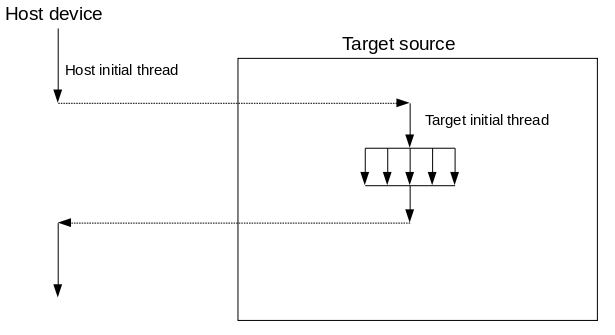
\includegraphics[width=\textwidth]{heter_1}
\centering
\captionsetup{justification=centering, singlelinecheck=false}
	\caption{Διάγραμμα ομάδων νημάτων σε ετερογενή αρχιτεκτονική}
\label{fig:heter_1}
\end{figure}

\subsubsection{H οδηγία \emph{\en{target teams}}}
\subparagraph{}
Η οδηγία \emph{\en{target teams}} κατασκευάζει μια ομάδα (\emph{\en{league}} που λειτουργούν σε έναν επιταχυντή. Κάθε μία από αυτές τις ομάδες είναι ένα αρχικό νήμα που εκτελεί παράλληλα την επόμενη δήλωση κώδικα. Η λειτουργία αυτή είναι παρόμοια με μια οδηγία \emph{\en{parallel}} με τη διαφορά ότι τώρα κάθε νήμα είναι μια ομάδα. Τα νήματα σε διαφορετικές ομάδες δεν μπορούν να συγχρονιστούν μεταξύ τους.

Όταν μια παράλληλη περιοχή συναντάται από μια ομάδα, κάθε αρχικό thread ομάδας γίνεται κύριο σε μια νέα υποομάδα. Το αποτέλεσμα είναι ένα σύνολο υποομάδων, οπου κάθε υποομάδα αποτελείται από ένα ή περισσότερο νήματα.

Αυτή η δομή χρησιμοποιείται για να εκφράζεται ένας τύπος χαλαρού παραλληλισμού, όπου ομάδες νημάτων εκτελούν παράλληλα, αλλά με μικρή αλληλεπίδραση μεταξύ των υποομάδων.


\subsubsection{Μοντέλο μνήμης ετερογενούς αρχιτεκτονικής}
\subparagraph{}

\paragraph{Η φράση \emph{\en{map}}}
\subparagraph{}
Τα νήματα που εκτελούνται σε έναν επιταχυντή μπορούν να έχουν ιδιωτικές μεταβλητές. Το κύριο νήμα που ξεκινά την εκτέλεση μιας παράλληλης περιοχής λαμβάνει μια ιδιωτική μεταβλήτη που εμφανίζεται στη φράση \emph{\en{private}} ή \emph{\en{firstprivate}} στην οδηγία \emph{\en{target}}.

Η φράση \emph{\en{map}} χρησιμοποιείται για τον διαμοιρασμό κοινής μνήμης από τον \emph{\en{host}} στον επιταχυντή. Οταν οι δυο συσκευές δεν έχουν κοινόχρηστη μνήμη, η μεταβλητή αντιγράφεται στον επιταχυντή. Η φράση \emph{\en{en}} αποκρύπτει αν η μεταβλητή μοιράζεται ή αντιγράφεται στη συσκευή στόχου. Το \emph{\en{OpenMP}} ενεργεί ανάλογα με την αρχιτεκτονική που χρησιμοποιείται.
\\

\begin{table}[htbp]
\captionsetup{justification=raggedright,
singlelinecheck=false
}
\caption{Ενέργειες που απαιτούνται στο \en{\emph{map}} ανάμεσα σε διαμοιραζόμενη και κοινόχρηστη μνήμη}
\def\arraystretch{1.5}
\begin{tabular}{| p{0.25\textwidth} | p{0.25\textwidth}|  p{0.25\textwidth} |  p{0.25\textwidth}|}
 Τύπος Μνήμης\cellcolor[HTML]{D0D0D0} & \textbf{\en{memory allocation}} \cellcolor[HTML]{D0D0D0} & \textbf{\en{copy}}\cellcolor[HTML]{D0D0D0} & \textbf{\en{flush}} \cellcolor[HTML]{D0D0D0} \\
\hline
\textbf{Διαμοιρασμένη} & Ναι & Ναι & Ναι \\
\hline
\textbf{Κοινόχρηστη} & Οχι & Οχι & Ναι \\
\hline
\end{tabular}
\end{table}

\paragraph{Περιβάλλον δεδομένων συσκευής}
\subparagraph{}
Ο επιταχυντής έχει ένα περιβάλλον μνήμης που περιέχει το σύνολο των μεταβλητών που είναι προσβάσιμες από νήματα που εκτελούνται σε αυτή τη συσκευή. Η αντιστοίχιση των δεδομένων διασφαλίζει ότι η μεταβλητή βρίσκεται στο περιβάλλον δεδομένων του επιταχυντή.

Μία μεταβλητής του εξυπηρετητή, αντιστοιχίζεται στην αντίστοιχη μεταβλητή του περιβάλλοντος δεδομένων του επιταχυντή.
Ανάλογα με τη διαθεσιμότητα της κοινόχρηστης μνήμης μεταξύ του εξυπηρετητή \emph{\en{host}} και της συσκευής προορισμού, η πρωτότυπη μεταβλητή του εξυπηρετητή και η αντίστοιχη μεγαβλητή της συσκευής προορισμού είναι είτε η ίδια μεταβλητή που βρίσκεται στη κοινόχρηστη μνήμη ή βρίσκεται σε διαφορετικές θέσεις, με αποτέλεσμα να απαιτούνται εργασίες αντιγραφής και ενημέρωσης για να διατηρηθεί η συνέπεια μεταξύ των δυο θέσεων.

Η ελαχιστοποίηση της μεταφοράς δεδομένων ανάμεσα στον εξυπηρετητή και τον επιταχυντή, αποτελεί κρίσιμο σημείο για την επίτευξη καλύτερης επίδοσης στις ετερογενείς αρχιτεκτονικές.
Η επαναληπτική αντιστοίχιση μεταβλητών που επαναχρησιμοποιούνται είναι αναποτελεσματική.

\paragraph{Δείκτες μεταβλητών συσκευής}
\subparagraph{}
Αν ο εξυπηρετητής και ο επιταχυντής δεν μοιράζονται τη κοινόχρηστη μνήμη, οι τοπικές μεταβλητές τους βρίσκονται σε διαφορετικές θέσεις μνήμης. Οταν μια μεταβλητή αντιστοιχίζεται στο περιβάλλον δεδομένων ενός επιταχυντή, γίνεται μια αντιγραφή και η καινούργια μεταβλήτή ειναι διαφορετική από την μεταβλητή του εξυπηρετητή.

Οι διευθύνσεις μνήμης αποθηκεύονται σε μεταβλητές που ονομάζονται δείκτες (\emph{\en{pointers}}. Ένα νήμα του εξυπηρετητή δε μπορεί να έχει πρόσβαση σε μνήμη μέσω ενός δείκτη που περιέχει διεύθυνση μνήμης του επιταχυντή. Ακόμη, ο επιταχυντής και ο εξυπηρετητής μπορεί να έχουν διαφορετική αρχιτεκτονική, δηλαδή ένας τύπος μεταβλητής μπορεί να είναι διαφορετικού μεγέθους ανάμεσα στις δύο συσκευές.

Ο δείκτης συσκευής \emph{\en{(device pointer)}} είναι ένας δείκτης που αποθηκεύεται στον εξυπηρετητή και περιέχει την διεύθυνση μνήμης στο περιβάλλον δεδομένων του επιταχυντή.


\selectlanguage{english}
\begin{lstlisting}[language=C++, caption={\el{Παράδειγμα} taskwait} , frame=tlrb]{Name}
int device = omp_get_default_device();
char *device_ptr = omp_target_alloc(n, device);
#pragma omp target is_device_ptr (device_ptr)
for (int j=0; j<n ; j++)
	*device_ptr++ = 0;
\end{lstlisting}
\selectlanguage{greek}
Εχω θέμα το \en{add vector doubles c10}.
\clearpage


\subsubsection{Η οδηγία \en{target}}
\subparagraph{}
Σκοπός της οδηγίας \en{target} είναι η μεταφορά και εκτέλεση ενός τμήματος κώδικα στον επιταχυντή. Η εκτέλεση γίνεται από ένα αρχικό νήμα στη συσκευή. Σε περίπτωση έλλειψης επιταχυντή στο σύστημα, ο κώδικας που προορίζεται να εκτελεστεί εκεί μέσω της οδηγίας \emph{\en{target}} θα εκτελεστεί στον εξυπηρετητή.

\selectlanguage{english}
\begin{lstlisting}[language=C++, caption={\el{Σύνταξη οδηγίας} target} , frame=tlrb]{Name}
#pragma omp target [clause[[,] clause]...]
\end{lstlisting}
\selectlanguage{greek}

\selectlanguage{english}
\begin{lstlisting}[language=C++, caption={\el{Παράδειγμα εκτέλεσης στον επιταχυντή} } , frame=tlrb]{Name}
void test() {
	int flag = 0;
	#pragma omp target map(flag)
	{
		flag = !omp_is_initial_device() ? 1 : 2;
	}
	if (flag == 1) {
		printf("Running on accelerator\n");
	} else if (flag == 2) {
		printf("Running on host\n");
	}
}
\end{lstlisting}
\selectlanguage{greek}

Η οδηγία \emph{\en{target}} δημιουργεί μια διεργασία που εκτελείται στον επιταχυντή. Η διεργασία για τον εξυπηρετητή ολοκληρώνεται όταν ολοκληρωθεί η εκτέλεση στον επιταχυντή. Οι φράσεις \emph{\en{nowait}} και \emph{\en{depend}} επηρεάζουν τον τύπο και την ασύγχρονη συμπεριφορά της διεργασίας. Από προεπιλογή, η διεργασίες στόχου είναι συγχρονισμένη. Το νήμα που τη συναντά περιμένει μέχρι την ολοκλήρωση της εκτέλεσής της.

Οι δείκτης μεταβλητών που εισάγονται στη φράση \emph{\en{map}}, είναι ιδιωτικές (\emph{\en{private}}) μέσα στη συσκευή στόχου. Οι ιδιωτικές μεταβλητές δείκτη διεύθυνσης αρχικοποιούνται με την τιμή της διεύθυνσης του επιταχυντή.

\clearpage

\selectlanguage{english}
\begin{lstlisting}[language=C++, caption={\el{Φράσεις οδηγίας} \emph{\en{target}} } , frame=tlrb]{Name}
if (/target:] scalar-expression)
map ([[map-type-modifier[,JJ map-type:] list]
device (integer-expression)
private (list)
firstprivate (list)
is_device_ptr (list)
defaultmap( tofrom:scalar)
nowait
depend ( dependence-type: list)
\end{lstlisting}
\selectlanguage{greek}

\subsubsection{Η οδηγία \en{target teams}}
\subparagraph{}
Η οδηγία \emph{\en{target teams}} καθορίζει την δημιουργία μια συστάδα αρχικών νημάτων όπου κάθε αρχικό νήμα αποτελεί και μια ομάδα. Κάθε αρχικό νήμα εκτελεί την περιοχή παράλληλα.

\begin{figure}[h]
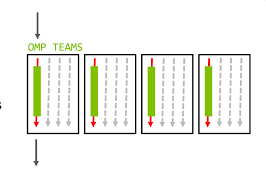
\includegraphics[width=0.75\textwidth]{target_teams}
\centering
\captionsetup{justification=centering, singlelinecheck=false}
	\caption{Ομάδες νημάτων με την οδηγία \emph{\en{target teams \cite{target_teams}}}}
\label{fig:target_teams}
\end{figure}


\selectlanguage{english}
\begin{lstlisting}[language=C++, caption={\el{Φράσεις οδηγίας} \emph{\en{target}} } , frame=tlrb]{Name}
num_teams (integer-expression)
threadJimit (integer-expression)
default(shared I none)
private (list)
firstprivate (list)
shared (list)
reduction (reduction-identifier : list)
\end{lstlisting}
\selectlanguage{greek}

\subsubsection{Η οδηγία \en{distribute}}
\subparagraph{}


\selectlanguage{english}
\begin{lstlisting}[language=C++, caption={\el{Σύνταξη οδηγίας} \emph{\en{distribute}} } , frame=tlrb]{Name}
#pragma omp distribute {clause[[,} clause}. . . j
	for-loops
\end{lstlisting}
\selectlanguage{greek}


\selectlanguage{english}
\begin{lstlisting}[language=C++, caption={\el{Φράσεις υποστηριζόμενες από την οδηγία} \emph{\en{distribute}} } , frame=tlrb]{Name}
private {list)
firstprivate {list)
lastprivate {list)
collapse (n)
dist_schedule {kind[, chunk_sizej)
\end{lstlisting}
\selectlanguage{greek}

Η οδηγία  \emph{\en{distribute}} καθορίζει τον διαμοιρασμό  επαναλήψεων ενός βρόγχου στα αρχικά νήματα των ομάδων που δημιουργήθηκαν από την οδηγία \emph{\en{target teams}}. Οι επαναλήψεις του βρόγχου χωρίζονται σε τμήματα και μοιράζονται στα κύρια νήματα των ομάδων. Η οδηγία \emph{\en{distribute}} δεν εχει υπονοούμενο φράγμα εργασιών στο τέλος της, πράγμα που σημαίνει οτι τα κύρια νήματα των ομάδων δε συγχρονίζονται στο τέλος της οδηγίας.

Η φράση \emph{\en{distschedule}} καθορίζει τον τρόπο που διαμοιράζονται οι επαναλήψεις σε τμήματα. Συγκριτικά με την οδηγία \emph{\en{for}} η \emph{\en{distribute}} έχει δυνατότητες για καλύτερη απόδοση. Ο μεταγλωττιστής μπορεί να πετύχει μεγαλύτερη βελτιστοποίηση.



\subsubsection{Σύνθετες οδηγίες επιταχυντών}
\subparagraph{}

Οι συνδυασμένες οδηγίες είναι ισοδύναμες με τις επιμέρους. Για παράδειγμα η οδηγία \emph{\en{parallel for}} έχει την ιδια σημασία με την \emph{\en{parallel}} ακολουθούμενη από την οδηγία \emph{\en{for}}. Παρόλα αυτά, ορισμένες φορές, οι συνδυασμένες οδηγίες μπορούν να επιτύχουν καλύτερες επιδόσεις.
Σε αυτή την παράγραφο, οι οδηγίες χωρίζονται σε δύο κατηγορίες, τις συνδυασμένες με \emph{\en{target}} και αυτές που συνδυάζονται με \emph{\en{target teams}}.

\selectlanguage{english}
\begin{lstlisting}[language=C++, caption={\el{Συνδυασμένες οδηγίας επιταχυντή}} , frame=tlrb]{Name}
#pragma omp target parallel [clause[[,] clause]...]
	structured block

#pragma omp target parallel for [clause[[,] clause]...]
	for-loops
	
#pragma omp target parallel for simd [clause[[,] clause]...]
	for-loops
	
#pragma omp target simd [clause[[,] clause]...]
	for-loops
\end{lstlisting}
\selectlanguage{greek}


\selectlanguage{english}
\begin{lstlisting}[language=C++, caption={\el{Συνδυασμένες οδηγίας επιταχυντή}} , frame=tlrb]{Name}
#pragma omp distribute parallel for [clause[[,] clause]...]
	for-loops
#pragma omp distribute simd [clause[[,] clause]...]
	for-loops
#pragma omp distribute parallel for simd [clause[[,] clause]...]
	for-loops
\end{lstlisting}
\selectlanguage{greek}


\subsubsection{Φράσεις οδηγίας \emph{\en{map}}}
\subparagraph{}
\selectlanguage{english}
\begin{lstlisting}[language=C++, caption={\el{Σύνταξη οδηγίας} map} , frame=tlrb]{Name}
map ([[map-type-modifier[,}} map-type:} list)

\end{lstlisting}
\selectlanguage{greek}
\selectlanguage{english}
\begin{lstlisting}[language=C++, caption={\el{Αποδεκτές τιμές για το } map-type} , frame=tlrb]{Name}
	alloc
	to
	from
	tofrom -> default
	release
	delete
\end{lstlisting}
\selectlanguage{greek}

Υπάρχουν τρεις φάσεις στην αντιστοίχιση μεταβλητών στον επιταχυντή:
\begin{enumerate}
  \item Η φάση \emph{\en{map-enter}} στην αρχή της εκτέλεσης της οδηγίας \emph{\en{target}}, όπου οι μεταβλητή αντιστοιχίζεται στον επιταχυντή. Σε αυτή τη φάση δεσμεύεται μνήμη του επιταχυντή για την αποθήκευση της μεταβλητής, και αντιγράφεται από τον εξυπηρετητή.
  \item Η φάση υπολογισμού που προκύπτει όταν, κατά τη διάρκεια εκτέλεσης της παράλληλης περιοχής, τα νήματα που εκτελούν το πρόγραμμα αποκτούν πρόσβαση στην αντιστοιχισμένη μεταβλητή.
  \item Η φάση εξόδου όπου ολοκληρώνεται η αντιστοίχιση των μεταβλητών στον επιταχυντή. Η τιμή της μεταβλητής στον επιταχυντή αντιγράφεται στην αντίστοιχη θέση του εξυπηρετητή. Η δεσμευμένη μνήμη του επιταχυντή ελευθερώνεται.
\end{enumerate}

Οι φάσεις 1 και 3 διαχειρίζονται την αποθήκευση και αντιγραφή των μεταβλητών ανάμεσα σε δυο συσκευές. Ο τύπος της αντιστοίχισης επηρεάζει την αντιγραφή μεταβλητών στον επιταχυντή ή τον εξυπηρετητή. Ο καθορισμός του τύπου αντιστοίχισης επηρεάζει την απόδοση του κώδικα.


\begin{table}[htbp]
\captionsetup{justification=raggedright,
singlelinecheck=false
}
\caption{Απαιτούμενη αντιγραφή για κάθε τύπο μεταβλητής κατά τις φάσεις εισόδου-εξόδου}
\def\arraystretch{1.5}
\begin{tabular}{| p{0.25\textwidth} | p{0.25\textwidth}|  p{0.25\textwidth} |  p{0.25\textwidth}|}
 \en{map-type}\cellcolor[HTML]{D0D0D0} & \textbf{Είσοδος} \cellcolor[HTML]{D0D0D0} & \textbf{Έξοδος}\cellcolor[HTML]{D0D0D0} \\
\hline
\textbf{\en{alloc}} & Οχι & Οχι \\
\hline
\textbf{\en{to}} & Ναι & Οχι \\
\hline
\textbf{\en{from}} & Οχι & Ναι \\
\hline
\textbf{\en{tofrom}} & Ναι & Ναι \\
\hline
\textbf{\en{release}} & - & Οχι \\
\hline
\textbf{\en{delete}} & - & Οχι \\
\hline
\end{tabular}
\end{table}

\clearpage
\selectlanguage{english}
\begin{lstlisting}[language=C++, caption={\el{Παράδειγμα χρήσης τύπου αντιστοίχισης μεταβλητών}} , frame=tlrb]{Name}
void foo(double A[1024], double B[1024], double C[1024) {
	#pragma omp target map(from : A) map(to: B) 
			map(alloc: C) // map enter
	{
		//CODE
	} // map exit
}
\end{lstlisting}
\selectlanguage{greek}

Στο προηγούμενο παράδειγμα:

Η μεταβλητή \textbf{Α}:
\begin{itemize}
  \item Δεν αρχικοποιείται στον επιταχυντή
  \item Οι τιμή της αντιγράφεται στον εξυπηρετητή
  \item Η μνήμη αποδεσμεύεται κατά την επιστροφή στον εξυπηρετητή.
\end{itemize}
\ \\
Η μεταβλητή \textbf{Β}:
\begin{itemize}
  \item Οι τιμή της αντιγράφεται στον επιταχυντή.
  \item Η μνήμη αποδεσμεύεται κατά την επιστροφή στον εξυπηρετητή.
\end{itemize}
\ \\
Η μεταβλητή \textbf{\en{C}}:
\begin{itemize}
  \item Οι τιμή της αντιγράφεται στον επιταχυντή.
  \item Η μνήμη αποδεσμεύεται κατά την επιστροφή στον εξυπηρετητή.
\end{itemize}

\subsubsection{Οδηγία \emph{\en{declare target}}}
\subparagraph{}
Η οδηγία \emph{\en{declare target}} χρησιμοποιείται για συναρτήσεις και μεταβλητής. Μια συνάρτηση που καλείται μέσα στο τμήμα του \emph{\en{target}} κώδικα, θα πρέπει να δηλώνεται στην οδηγία \emph{\en{declare target}}. Ακόμη, η οδηγία χρησιμοποιείται για την αντιστοίχιση \emph{\en{global}} μεταβλητών στο περιβάλλον δεδομένων του επιταχυντή.



\selectlanguage{english}
\begin{lstlisting}[language=C++, caption={\el{Συνδυασμένες οδηγίας επιταχυντή}} , frame=tlrb]{Name}
#pragma omp declare target
	declarations-definitions-seq
#pragma omp end declare target
#pragma omp declare target(extended-list)
#pragma omp declare target clause[[l] clause]...]

CLAUSE:
to (extended-list)
link (list)
\end{lstlisting}
\selectlanguage{greek}

\textbf{\en{TODO}} έχει και αλλο.
